% -*- mode: noweb; noweb-default-code-mode: R-mode; -*-
\documentclass[9pt]{beamer}
\usepackage{graphicx}

\title{Visualizing multivariate data using lattice and latticedl\\
http://directlabels.r-forge.r-project.org}
\author{Toby Dylan Hocking}
\date{15 October 2009}

\AtBeginSection[]
{
  \begin{frame}<beamer>
    \frametitle{Outline}
    \tableofcontents[currentsection]
  \end{frame}
}

\AtBeginSubsection[]
{
  \begin{frame}<beamer>
    \frametitle{Outline}
    \tableofcontents[currentsection,currentsubsection]
  \end{frame}
}

\newcommand{\framet}[2]{\frame{
\begin{itemize}
\frametitle{#1}{#2}
\end{itemize}
}}

\newcommand{\picframe}[1]{
  \frame[plain]{
    \includegraphics[width=\textwidth]{#1}
  }
}

\usepackage{Sweave}
\begin{document}
\setkeys{Gin}{width=\textwidth}
\frame{\titlepage}

\section{lattice}

\frame[containsverbatim]{\frametitle{Load some data}
\begin{Schunk}
\begin{Sinput}
> data(Chem97, package = "mlmRev")
> head(Chem97)
\end{Sinput}
\begin{Soutput}
  lea school student score gender age gcsescore   gcsecnt
1   1      1       1     4      F   3     6.625 0.3393157
2   1      1       2    10      F  -3     7.625 1.3393157
3   1      1       3    10      F  -4     7.250 0.9643157
4   1      1       4    10      F  -2     7.500 1.2143157
5   1      1       5     8      F  -1     6.444 0.1583157
6   1      1       6    10      F   4     7.750 1.4643157
\end{Soutput}
\end{Schunk}
}

\frame[containsverbatim]{\frametitle{Simple histogram}
\begin{Schunk}
\begin{Sinput}
> library(lattice)
> histogram(~gcsescore, Chem97)
\end{Sinput}
\end{Schunk}
\includegraphics{HOCKING-latticedl-semin-r-002}
}
\frame[containsverbatim]{\frametitle{Conditional histogram}
\begin{Schunk}
\begin{Sinput}
> histogram(~gcsescore | factor(score), xlab = "some label", 
+     main = "a big title that takes up a whole line and then some", 
+     ylab = "another label", Chem97)
\end{Sinput}
\end{Schunk}
\includegraphics{HOCKING-latticedl-semin-r-003}
}
\section{latticeExtra}

\section{latticedl}

\framet{Direct labels are almost always better than legends}{
\item Edward Tufte, professor emeritus of Statistics at Yale
\item 1983, The Visual Display of Quantitative Information
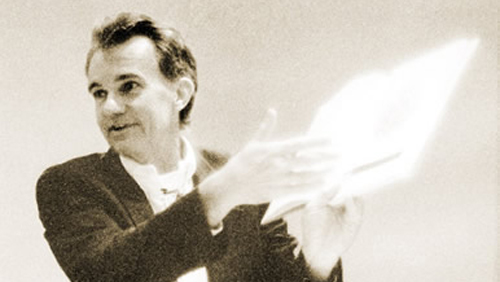
\includegraphics{TUFTE.jpg}}

\end{document}

Sinput